\documentclass{article}

\usepackage{graphicx}
\usepackage{tikz}
\usepackage{tikzsymbols}
\usetikzlibrary{calc,patterns,shapes.geometric}
\pagestyle{empty}
\usepackage[margin=0pt]{geometry}
\geometry{papersize={14in,12in}}

\def\centerarc[#1](#2)(#3:#4:#5){\draw[#1] ($(#2)+({#5*cos(#3)},{#5*sin(#3)})$) arc (#3:#4:#5);}

\begin{document}
	\begin{figure}
		\centering
		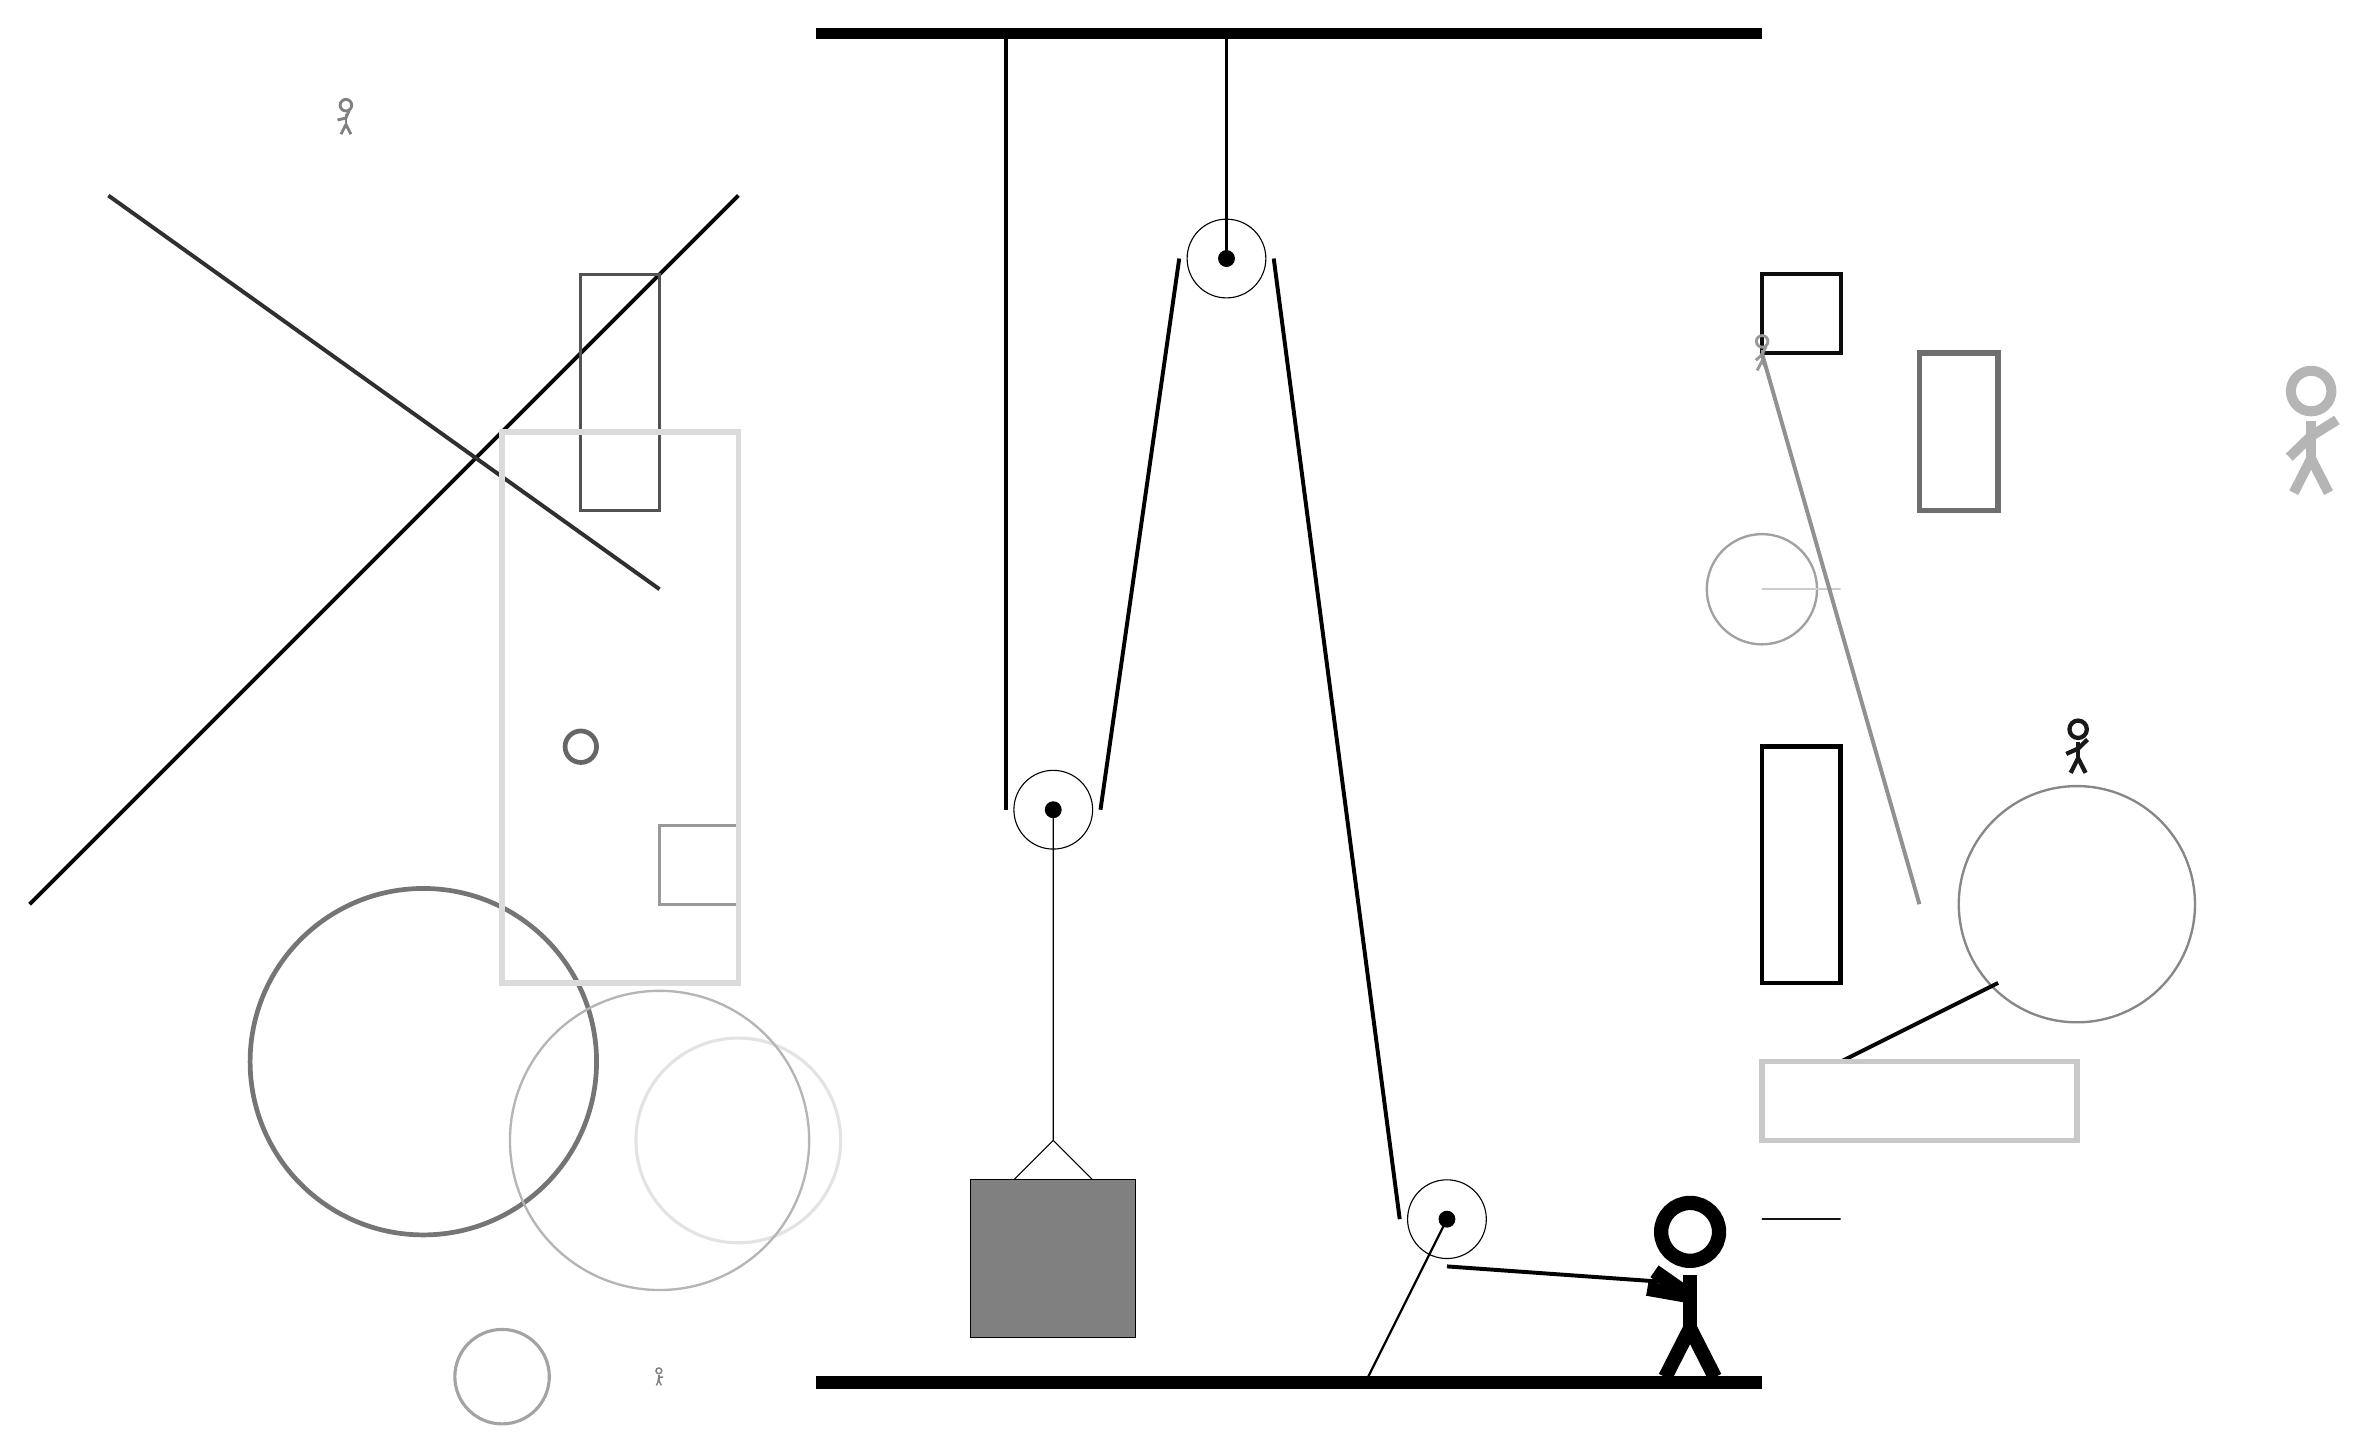
\begin{tikzpicture}
			%%%%% START %%%%%
			
			\draw[fill=black] (-2, 14) rectangle (10, 14.125);
			
			\draw (3.2, 11.2) circle (0.5);
			\draw[fill=black] (3.2, 11.2) circle (0.1);
			\draw[thick] (3.2, 11.2) -- (3.2, 14);
			
			\draw (6, -1) circle (0.5);
			\draw[fill=black] (6, -1) circle (0.1);
			\draw[thick] (6, -1) -- (5, -3);
			
			\draw (1, 4.2) circle (0.5);
			\draw[fill=black] (1, 4.2) circle (0.1);
			
			\draw[line width=0.5mm, color=black!95] (10, 10) rectangle (11, 11);
			
			\draw [line width=0.3mm, color=black!37](10, 7) circle (0.7);
			\node[line width=0.3mm, color=black!29] at (17, 9) {\Strichmaxerl[7][44][32]};
			\draw[line width=0.2mm, color=black!20] (10, 7) rectangle (11, 7);
			\draw [line width=0.3mm, color=black!47](14, 3) circle (1.5);
			
			\draw [line width=0.4mm, color=black!36](-6, -3) circle (0.6);
			
			\draw[line width=0.5mm, color=black!97](13, 2) -- (11, 1);
			\draw[line width=0.4mm, color=black!40] (-4, 3) rectangle (-3, 4);
			\draw[line width=0.6mm, color=black!94] (-3, 4) rectangle (-3, 8);
			\draw[line width=0.6mm, color=black!100] (10, 2) rectangle (11, 5);
			\node[line width=0.2mm, color=black!40] at (10, 10) {\Strichmaxerl[2][44][63]};
			\draw[line width=0.5mm, color=black!97](-3, 12) -- (-12, 3);
			\draw [line width=0.4mm, color=black!11](-3, 0) circle (1.3);
			
			\node[line width=0.3mm, color=black!90] at (14, 5) {\Strichmaxerl[3][24][44]};
			\draw[line width=0.7mm, color=black!57] (12, 10) rectangle (13, 8);
			\draw[line width=0.5mm, color=black!43](12, 3) -- (10, 10);
			
			\node[line width=0.2mm, color=black!50] at (-4, -3) {\Strichmaxerl[1][78][2]};
			\node[line width=0.4mm, color=black!50] at (-8, 13) {\Strichmaxerl[2][13][67]};
			\draw[line width=0.3mm, color=black!92] (11, -1) rectangle (10, -1);
			
			\draw[line width=0.5mm, color=black!81](-4, 7) -- (-11, 12);
			\draw [line width=0.4mm, color=black!90](-5, 5) circle (0.2);
			
			\draw [line width=0.6mm, color=black!54](-7, 1) circle (2.2);
			
			\draw[line width=0.4mm, color=black!68] (-4, 11) rectangle (-5, 8);
			\draw [line width=0.6mm, color=black!60](-5, 5) circle (0.2);
			\draw[line width=0.7mm, color=black!14] (-3, 2) rectangle (-6, 9);
			
			\draw [line width=0.3mm, color=black!29](-4, 0) circle (1.9);
			\draw[line width=0.7mm, color=black!21] (10, 0) rectangle (14, 1);
			
			\draw (1, 4.2) -- (1, 0) -- (0.5, -0.5);
			\draw (1, 0) -- (1.5, -0.5);
			\draw[fill=black!50] (-0.05, -0.5) rectangle (2.05, -2.5);
			
			\draw[line width=0.5mm] (0.4, 14) -- (0.4, 4.2);
			\centerarc[line width=0.5mm](1, 4.2)(180:360:0.6);
			\draw[line width=0.5mm](1.6, 4.2) -- (2.6, 11.2);
			\centerarc[line width=0.5mm](3.2, 11.2)(0:180:0.6);
			\draw[line width=0.5mm](3.8, 11.2) -- (5.4, -1);
			\centerarc[line width=0.5mm](6, -1)(180:270:0.6);
			\draw[line width=0.5mm](6, -1.6) -- (8.8, -1.8);
			
			\node at (9, -1.9) {\Strichmaxerl[10][-35][170]};
			
			\draw[fill=black] (-2, -3) rectangle (10, -3.15);
			
			%%%%% END %%%%%
		\end{tikzpicture}
	\end{figure}	
\end{document}